\documentclass[11pt]{article}
\usepackage[margin= 1in]{geometry}
% insert a picture
%\begin{Figure}[H]
% \centering
%\includegraphics[scale=2,angle=30][width=0.5\textwidth]{fig1/Treemap2.png}
% %\vspace{-0.1 in}
%  \caption{The Tree map of April 1st shows a less anomalous situation where the magnitudes of different servers may be close. Tree map rectangles with smaller sizes (left) could also be viewed via a zoom and pan interaction with respect to blocks on the right.}
% \label{Fig:treemap2}
% \vspace{-0.1 in}
%\end{figure}

%insert a table
%\begin{table}
%\begin{tabular}{|l|l|l|}
%\hline
%h1&h2&h3\\
%\hline
%a&b&c\\
%\hline
%\end{tabular}
%\end{table}
\usepackage{cite,url,mathptmx,times,amsmath,algorithm,algorithmic,cases,subFig,multirow}
\usepackage{graphicx}
\usepackage{grffile}
\usepackage{indentfirst}
\usepackage{tabularx}
\begin{document}
\title{Analysis of Climatological Data}
\author{Xiaoying Yu\\Central Michigan University\\yu3x@cmich.edu
\and Ting Li\\Central Michigan University\\li2t@cmich.edu
\and Hesham Salman\\Central Michigan University\\hesham8@gmail.com}
\maketitle
\newpage
\begin{abstract}
\end{abstract}
\newpage
\section{Introduction}
Climate is a term for describing the average conditions in a long period. Annual Climatological Summaries offer valuable information to researchers over thousands of reporting in the United States. Much attributes are collected to form the climatical data, such as temperature, precipitation, longitude, latitude, location, location name, and so on. These data stimulates researchers to dig out much useful information to predict the weather changing.

The data set that we discuss is from National Oceannic And Atmospheric Administration(NOAA)\cite{center2010national}. NOAA collects the whole data from daily weather forecasts, severe storm warnings and climate monitoring to fisheries management, coastal restoration and supporting marine commerce\cite{center2010national}.  There are several attributes in the data set, such as station, station name, elvation, latitude, longitude, date, the departure from normal monthly temperature(DPNT), the departure from normal monthly precipitation(DPNP), number days in month with maximum temperature greater than or equal 90 F(DT90), number days in month with maximum temperature less than or equal 32 F(Dx32). This data covers more than 5,000 stations in United Stated, and it records the report data from January in 2014 to November in 2014 of every station.

As for the data set, we hypothesized that elevation had some bearing relationship on the departure from normal temperature or precipitation. Basing on the hypothesis, we take several steps to testify it, for example, cleaning the noisy data, normalizing the data, finding the associational rule of elevation and DPNT, an the associational rule of elevation and DPNP, classifying the data, finding the cluster of the data. To be specific, we also use Java to clean and normalize the big data, which has 62,503 tuples. In the classification, we randomly choose 63\% of the data to build a classifier, and then test the rest data. When referring to this step, we also apply python to converting a comma-separated values(CSV) file to aircraft rescue and firefighting(ARFF) file. In the visualization, we applied Data-Driven Documents JavaScript to visualization the relationship of the association rules. The main tool that we use to find the association rules, classification, and clustering, we apply the weka that is a collection of machine learning algorithms for data mining tasks\cite{hall2009weka}. We concluded several findings. First of all, elevation does have an effect on precipitation: as elevation increase, precipitation tends to normalize. Secondly, when the elevation is normal, most of the monthly DPNT or DPNP tend to be normal.

In the following sections, the first section introduces the data cleaning and normalization. The next section explains how to get the association rules and the visualization of the rules. Then we discuss the classification process basing on five attributes, which are longitude, latitude, DPNT, DPNP, elevation. Furthermore, we also fucus on the clustering to find out the cluster of elevation and DPNT, and the cluster of elevation and DPNP. Finally, we summarized the result that we get from the project.


\section{Data Cleaning and Normalization}
The data we have has nine attributes that were mentioned before, and every month has around 5642 records of different stations. As for the big database, we found there are 262 ``unknown'' value filled in the station, longitude, and latitude value sets, and 12,759 records contain ``-9999'' value in the DPNT or DPNP or both. The total data tuples reach to 62,053. In other words, the percentage of the missing value is $( 262 + 12759 ) / 62053 * 100\% = 22\% $.
\subsection{Data Cleaning}
With the missing data of the first instance, we choose Complete-case method\cite{han2006data}. That is, 262 ``unknown'' tuples are removed. As to the second instance, we refer to the annual document from the NOAA. ``-9999'' was used to represent the missing value in the elevation, DPNT, and DPNP columns. For the correctness, we use Ad Hoc method to record all the ``-9999'' with ``0''. We use this method because DPNT and DPNP are the departure values. ``0'' will not produce big influence on the normalization.
\subsection{Data Normalization}
When we read the data, there is a big difference between the maximum value and the minimum value of these columns(elevation, DPNT, DPNP, longitude, latitude. According to this situation, we applied Z-score normalization method to normalize all these value sets. The Z-score equation is given in Equation \eqref{z-score}.
\begin{equation}
Z-score = \frac{v-\mu}{\delta} \label{z-score}
\end{equation}
where $\mu$ and $\delta$ are the mean and standard deviation of attribute v, respectively.

Specifically, each attribute was calculated in the following steps. First of all, the average of DPNT/DPNP/elevation/longitude/latitude are calculated as $\mu$. Secondly, we apply $|v-\mu|$ to calculate the absolute values of each attribute. Then, we get the average of these absolute values, which is taken as standard derivation $\delta$. Finally, we apply Equation\eqref{z-score} to calculate the Z-score.
After that, we classify five categories of each attribute. For example, elevation has normal, low, very low, high, very high status; DPNT has normal, cold, very cold, warm, very warm. As the normal status in this five attribute, we set the standard derivation of five attributes to the range of (-1, 1). Low or cold are usually set into the normalized range (-2, -1). The very low or very cold status are set the normalized number is less than -2. The same as the high/warm and very high/very warm, which are set into the normalized range (1,2) and greater than 2, respectively.
\section{Association}
After getting cleaning data for eleven mouths, what we have to do next is to find out whether elevation will have some bearings on temperature or precipitation; and if there are, will the effects be the same for each month?  Based on Association Rules in data mining and Weka software we are trying to confirm our hypothesis.
In Weka, we set our support level to 0.1 and the confidence value to 0.6. For each month, we pick up the association rules that include information about DPNP (departure from normal precipitation) or DPNT (departure from normal temperature) implied by Elevation.  Association rules found in January are given as an example in the following:

1.  DPNT Class= Very Cold 658 ==$>$  Elevation Class= Normal 633    conf:(0.96)

2.  DPNT Class= Cold  DPNP Class= Normal 705 ==$>$  Elevation Class= Normal 622    conf:(0.88)

3.  DPNT Class= Normal  Elevation Class= Normal 1624 ==$>$  DPNP Class= Normal 1392    conf:(0.86)

4.  DPNT Class= Cold 1047 ==$>$  Elevation Class= Normal 846    conf:(0.81)

5.  DPNT Class= Normal 2714 ==$>$  DPNP Class= Normal 2178    conf:(0.8)

6.  Elevation Class= Normal 3545 ==$>$  DPNP Class= Normal 2763    conf:(0.78)

7.  DPNT Class= Cold  Elevation Class= Normal 846 ==$>$  DPNP Class= Normal 622    conf:(0.74)

8.  DPNT Class= Cold 1047 ==$>$  DPNP Class= Normal 705    conf:(0.67)

9.  DPNP Class= Normal 4137 ==$>$  Elevation Class= Normal 2763    conf:(0.67)

10.  DPNT Class= Normal  DPNP Class= Normal 2178 ==$>$  Elevation Class= Normal 1392    conf:(0.64)

11.  Elevation Class= Low 965 ==$>$  DPNT Class= Normal 591    conf:(0.61)

In the above Associations rules, we try to find out Elevation\rq s effects on DPNP using the sixth rule and try to find out Elevation\rq s effects on DPNT basing on the eleventh one. After getting all of the similar interesting Association rules in each month, we combined them together and try to show those in Gantt Chart Visualizations, which are designed based on D3 JavaScript.

In Gantt chart, we show date information in the X-axis, on which, each interval represents a month in 2014 and there are eleven months in total.  Y-axis is used to show the Elevation information, as we already introduced in the Data Normalization part, we normalize our whole dataset’s elevation value into five classifications; they are very low, low, normal, high and very high. So in our Gantt chart Y-axis, there are five values in all, namely very low, low, normal, high and very high. In our case, DPNP and DPNT are showed in five colors, their relationship are showed in Table~\ref{table:DPNP-DPNT-COLOR}.

\begin{table}
\centering
\begin{tabularx}{\textwidth}{|X|X|X|}
  \hline
  \textbf{DPNP} & \textbf{DPNT} & \textbf{COLOR}\\
  \hline\hline
  Very Wet & Very Hot & Red\\
  \hline
  Wet & Hot & Yellow\\
  \hline
  Normal & Normal & Green\\
  \hline
  Dry & Cold & Blue \\
  \hline
  Very Dry & Very Cold & Black \\
  \hline

\end{tabularx}
\caption{DPNP,DPNT class values and their related color in Gantt Chart}
                \label{table:DPNP-DPNT-COLOR}
                \end{table}

According to the Association Rules that we gather from Weka, the relationship between Elevation and DPNP is summarized in Gantt Chart and the specific view is showed in Figure \ref{fig:Gantt Chart for DPNP}.

\begin{figure}
  \centering
  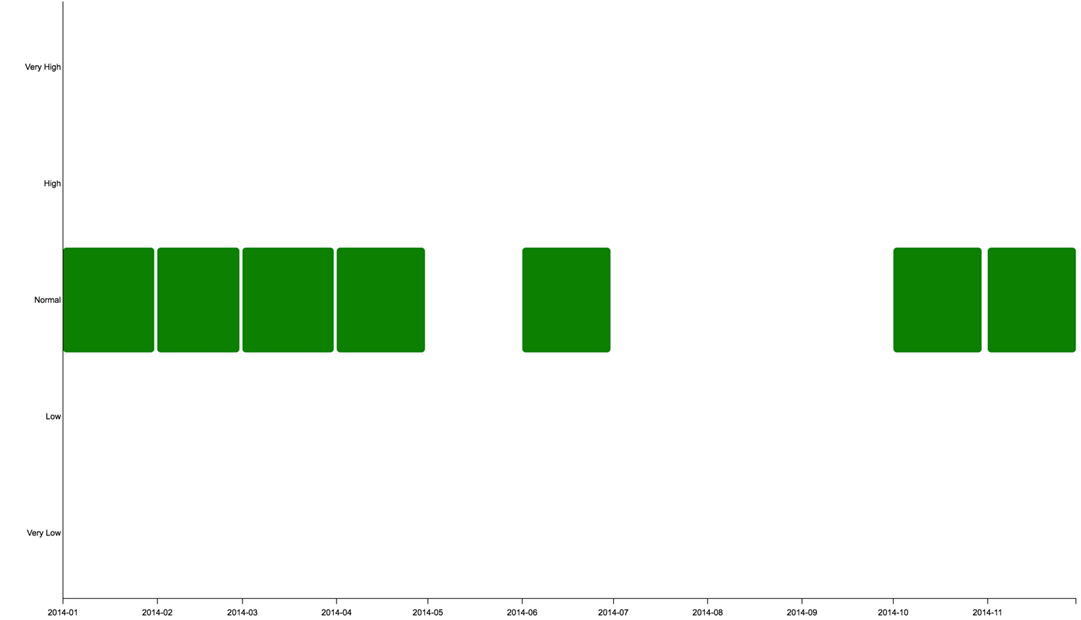
\includegraphics[width=\textwidth]{fig/ganttchart-dpnp.png}
  \caption{In Elevation-DPNP Cantt Chart, during January,February,March,April,June,October and November, at the places which have a Normal Elevation, their DPNP class values tend to be normal, and there are no association rules for May, July, Augus or September.}
  \label{fig:Gantt Chart for DPNP}
  \vspace{-0.1 in}
\end{figure}

As we can see from the Elevation-DPNP visualization, in most of the months, such as January, February and March, when the Elevation value is Normal, the DPNP value tends to be Normal too. Information in this visualization infers that for the locations which have a Normal elevation, their departure from normal precipitation and temperature tend to be Normal too.

We also showed the relationship between Elevation and DPNT in Gantt Chart, and the final result is presented in Figure \ref{fig:Gantt Chart for DPNT}.

\begin{figure}
  \centering
  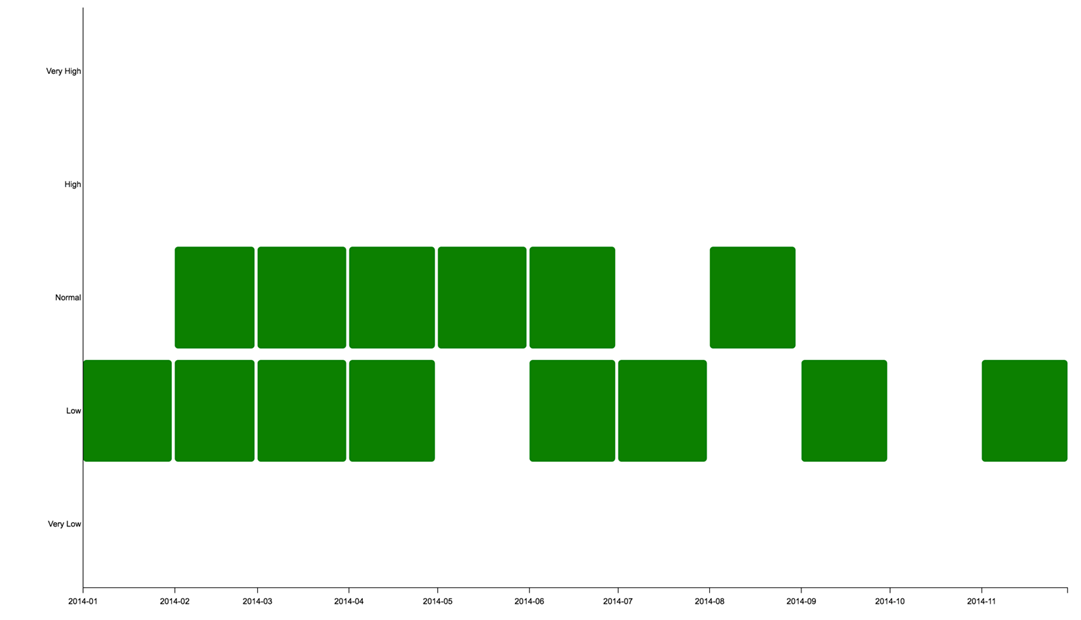
\includegraphics[width=\textwidth]{fig/ganttchart-dpnt.png}
  \caption{In Elevation-DPNT Cantt Chart,while location's Elevation is Low or Normal, its DPNT class value tends to be Normal}
  \label{fig:Gantt Chart for DPNT}
  \vspace{-0.1 in}
\end{figure}

\section{Classification}
Rules found in Association are only based on three attributes, namely Elevation, DPNP and DPNT.  Except for these rules, we want to find out some other interesting patterns from our dataset; hence, we take advantage of Classify in Weka software.  In the Classification, five attributes are under analysis; they are Elevation, Latitude, Longitude, DPNP and DPNT, what we want to find out is that whether we can make some predictions about certain location\rq s DPNP or DPNT value basing on its Elevation, Latitude, and Longitude.  Different from data processing in Association, in which we try to find Association Rules in each month separately; in Classification, we use java language to randomly select 63.2\% records in our whole dataset and treat them as training data , other left records are regarded as testing data.  In Weka Classify, we use the Decision Tree algorithm, set the confidenceFactor to 0.6, and we get the following results:

\subsection{DPNP}
There are 152 classifiers about DPNP in total, and among which,   44 indicates that some locations\rq DPNP class values are Very Wet or Very Dry, others locations are all keep normal.  In the 44 interesting classifiers, we find that in Partial South of America which have a low Elevation, while their DPNT class values are Very Warm, their DPNP class values tend to be Very Dry. The detailed classifiers information is showed as follows:

Elevation Class = Low---Latitude Class = Far South---DPNT Class = Very Warm---Longitude Class = Central:  Very Dry

Elevation Class = Low---Latitude Class = Far South---DPNT Class = Very Warm---Longitude Class = West:  Very Dry

Elevation Class = Low---Latitude Class = Far South---DPNT Class = Very Warm---Longitude Class = East:  Very Dry

Elevation Class = Low---Latitude Class = Far South---DPNT Class = Very Warm---Longitude Class = Far East:  Very Dry.

Hence, we can learn from these classifiers that places in Partial South of America, which have a Low elevation, they are becoming warmer and drier comparing to the previous 20 years’ normal temperature and precipitation.

Meanwhile, some other classifiers tell us that some places are becoming wetter, such as the following ones:

Elevation Class = Normal---Longitude Class = Far East--- DPNT Class = Warm--- Latitude Class = South:  Very Wet

Elevation Class = Normal---Longitude Class = Far East--- DPNT Class = Warm--- Latitude Class = North:  Very Wet

Elevation Class = Normal---Longitude Class = Far East--- DPNT Class = Warm--- Latitude Class = Far North:  Very Wet

As we can see that these places belong to South East or North East America, while their elevation class values are all Normal, their DPNT class values will be Warm.

\subsection{DPNT}

There are 126 classifiers in total, among these 126 classifiers, we find that 93 classifiers imply DPNT value is normal, and there are also some interesting classifiers we find from the result. Such as in North West or Central West of American, while the DPNP class is Very Dry, no matter the Elevation class is Low, Normal, High or Very high, their DPNT class values are all warm or very warm, which indicates that these place are becoming warmer and drier comparing to previous 20 years’ normal temperature and precipitation, the detailed classifiers are showed as following:

Longitude Class = West--- DPNP Class = Very Dry--- Latitude Class = North--- Elevation Class = Low:  Very Warm

Longitude Class = West--- DPNP Class = Very Dry--- Latitude Class = North--- Elevation Class = Very High:  Very Warm

Longitude Class = West--- DPNP Class = Very Dry--- Latitude Class = North--- Elevation Class = Normal:  Very Warm

Longitude Class = West--- DPNP Class = Very Dry--- Latitude Class = North--- Elevation Class = High:  Warm

Longitude Class = West--- DPNP Class = Very Dry--- Latitude Class = Central--- Elevation Class = Very High:  Warm

Longitude Class = West--- DPNP Class = Very Dry--- Latitude Class = Central--- Elevation Class = Normal:  Very Warm

Longitude Class = West--- DPNP Class = Very Dry--- Latitude Class = Central--- Elevation Class = High:  Very Warm


\section{Clustering}


\section{Conclusion}
When elevation is low or normal, DPNT tends to be normal. When elevation is normal, DPNP tends to be normal.

\section{Reference}
\bibliographystyle{plain}
\bibliography{bb}
\end{document}
